%Este trabalho está licenciado sob a Licença Atribuição-CompartilhaIgual 4.0 Internacional Creative Commons. Para visualizar uma cópia desta licença, visite http://creativecommons.org/licenses/by-sa/4.0/deed.pt_BR ou mande uma carta para Creative Commons, PO Box 1866, Mountain View, CA 94042, USA.

\chapter{Derivadas}\label{cap_deriv}
\thispagestyle{fancy}

\ifispython
\begin{obs}\normalfont{(Códigos \verb+Python+)}\label{obs:deriv_python}
  Nos códigos \verb+Python+ inseridos ao longo deste capítulos, estaremos assumindo o seguinte preâmbulo:
\begin{verbatim}
%matplotlib inline
from sympy import *
init_printing()
var('x',real=True)
\end{verbatim}
\end{obs}
\fi

\section{Retas tangentes e derivadas}\label{cap_deriv_sec_retg}

Definimos a {\bf reta secante} ao gráfico de uma dada função $f$ pelos pontos $x_0$ e $x_1$, $x_0\neq x_1$, como sendo a reta determinada pela equação
\begin{equation}
  y = \frac{f(x_1)-f(x_0)}{x_1-x_0}(x-x_0)+f(x_0).
\end{equation}
Isto é, é a reta que passa pelos pontos $(x_0,f(x_0))$ e $(x_1,f(x_1))$. Veja a Figura \ref{fig:retsectg}. Observemos que o coeficiente angular da reta secante é
\begin{equation}
  m_{\text{sec}} = \frac{f(x_1)-f(x_0)}{x_1-x_0}.
\end{equation}

\begin{figure}[H]
  \centering
  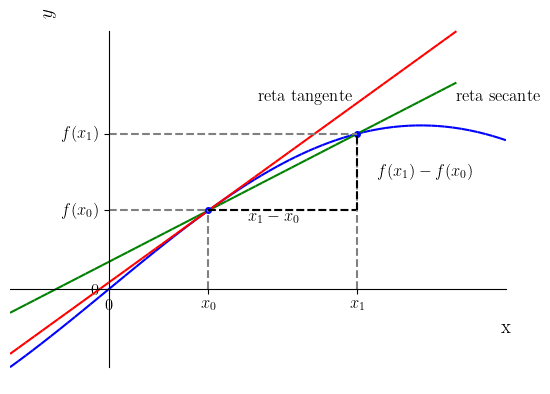
\includegraphics[width=0.7\textwidth]{./cap_deriv/dados/fig_retsectg/fig_retsectg}
  \caption{Esboços de uma reta secante (verde) e da reta tangente (vermelho) ao gráfico de uma função.}
  \label{fig:retsectg}
\end{figure}

A {\bf reta tangente} ao gráfico de uma função $f$ em $x=x_0$ é a reta que passa pelo ponto $(x_0, f(x_0))$ e tem coeficiente angular
\begin{equation}\label{eq:mtg}
  m_{\text{tg}} = \lim_{x_1\to x_0} \frac{f(x_1)-f(x_0)}{x_1-x_0}.
\end{equation}
Isto é, a reta de equação
\begin{equation}
  y = m_{\text{tg}}(x-x_0)+f(x_0).
\end{equation}
Menos formal, é a reta limite das retas secantes ao gráfico da função pelos pontos $x_0$ e $x_1$, quando $x_1\to x_0$. Veja a Figura \ref{fig:retsectg}.

\begin{obs}
  Fazendo $h = x_1-x_0$, temos que \eqref{eq:mtg} é equivalente a
  \begin{equation}
    m_{\text{tg}} = \lim_{h\to 0} \frac{f(x_0+h)-f(x_0)}{h}.
  \end{equation}
\end{obs}

\begin{ex}
  Seja $f(x)=x^2$ e $x_0 = 1$. O coeficiente angular da reta tangente ao gráfico de $f$ no ponto $x_0$ é
  \begin{align}
    m_{\text{tg}} &= \lim_{h\to 0} \frac{f(x_0+h)-f(x_0)}{h}\\
                  &= \lim_{h\to 0} \frac{(1+h)^2-1}{h}\\
                  &= \lim_{h\to 0} \frac{1+2h+h^2-1}{h}\\
                  &= \lim_{h\to 0} \frac{2+h}{1} = 2.
  \end{align}
  Assim sendo, a reta tangente ao gráfico de $f(x)=x^2$ no ponto $x_0=1$ tem coeficiente angular $m_{\text{tg}} = 2$ e equação
  \begin{equation}
    y = 2(x-1)+1 = 2x-1.
  \end{equation}
  \ifispython
  Com o \verb+SymPy+, podemos obter a reta tangente com os seguintes comandos:
\begin{verbatim}
h = symbols('h',real=True)
f = lambda x: x**2
x0 = 1
# coef. angular
mtg = limit((f(x0+h)-f(x0))/h,h,0)

# reta tangente
mtg*(x-x0)+f(x0)
\end{verbatim}
  \fi
\end{ex}

\subsection{A derivada em um ponto}

A {\bf derivada} de uma função $f$ {\bf em um ponto} $x=x_0$ é denotada por $f'(x_0)$ ou $\displaystyle \frac{\dd f}{\dd x}(x_0)$ e é definida por
\begin{equation}
  f'(x_0) = \frac{\dd f}{\dd x}(x_0) = \lim_{h\to 0} \frac{f(x_0+h)-f(x_0)}{h}.
\end{equation}

\begin{ex}
  Vejamos os seguintes casos:
  \begin{enumerate}[a)]
  \item $f(x) = k$, $k$ constante.
    \begin{align}
      f'(x_0) &= \lim_{h\to 0} \frac{f(x_0+h)-f(x_0)}{h}\\
              &= \lim_{h\to 0} \frac{k-k}{h} = 0.
    \end{align}
  \item $f(x) = x$.
    \begin{align}
      f'(x_0) &= \lim_{h\to 0} \frac{f(x_0+h)-f(x_0)}{h} \\
              &= \lim_{h\to 0} \frac{x_0+h-x_0}{h} = 1.
    \end{align}
  \item $f(x) = \sqrt{x}$, $x_0=1$.
    \begin{align}
      f'(1) &= \lim_{h\to 0} \frac{\sqrt{1+h}-1}{h}\\
            &= \lim_{h\to 0} \frac{\sqrt{1+h}-1}{h}\frac{\sqrt{1+h}+1}{\sqrt{1+h}+1}\\
            &= \lim_{h\to 0} \frac{1+h-1}{h(\sqrt{1+h}+1)} = \frac{1}{2}.
    \end{align}
  \end{enumerate}
\end{ex}

\subsection*{Exercícios}

\emconstrucao

\section{Função derivada}\label{cap_deriv_sec_deriv}

A {\bf derivada} de uma função $f$ em relação à variável $x$ é a função $\displaystyle f' = \frac{\dd f}{\dd x}$ cujo valor em $x$ é
\begin{equation}\label{eq:derivada}
  \lim_{h\to 0} \frac{f(x+h)-f(x)}{h},
\end{equation}
quando este limite existe. Dizemos que $f$ é {\bf derivável} (ou {\bf diferenciável}) em um ponto $x$ de seu domínio, quando o limite dado em \eqref{eq:derivada} existe. Se isso ocorre para todo número real $x$, dizemos que $f$ é derivável em toda parte.

\begin{ex}
  A derivada de $f(x) = x^2$ é
  \begin{align}
    f'(x) &= \lim_{h\to 0} \frac{f(x+h)-f(x)}{h}\\
          &= \lim_{h\to 0} \frac{(x+h)^2 - x^2}{h}\\
          &= \lim_{h\to 0} \frac{x^2+2xh+h^2-x^2}{h}\\
          &= \lim_{h\to 0} 2x+h = 2x.
  \end{align}
  \ifispython
  Com o \verb+SymPy+, podemos usar os seguintes comandos para verificarmos este resultado:
\begin{verbatim}
h = symbols('h',real=True)
f = lambda x: x**2
limit((f(x+h)-f(x))/h,h,0)
\end{verbatim}
  \fi
\end{ex}

\begin{obs}
  A derivada à direita (à esquerda) de uma função $f$ em um ponto $x$ é definida por
  \begin{equation}
    f_{\pm}'(x) = \frac{\dd f}{\dd x^{\pm}} = \lim_{h\to 0^\pm} \frac{f(x+h)-f(x)}{h}.
  \end{equation}
  Desta forma, no caso de pontos extremos do domínio de uma função, empregamos a derivada lateral correspondente.
\end{obs}

\begin{ex}
  A função valor absoluto é derivável para todo $x\neq 0$ e não é derivável em $x=0$. De fato, para $x<0$ temos
  \begin{align}
    f'(x) &= \lim_{x\to 0} \frac{|x+h|-|x|}{h}\\
          &= \lim_{h\to 0} \frac{-(x+h)+x}{h}\\
          &= \lim_{h\to 0} \frac{h}{h} = 1.
  \end{align}
  Analogamente, para $x>0$ temos
  \begin{align}
    f'(x) &= \lim_{x\to 0} \frac{|x+h|-|x|}{h}\\
          &= \lim_{x\to 0} \frac{x+h-x}{h}\\
          &= \lim_{x\to 0} \frac{h}{h} = 1.
  \end{align}
  Agora, para $x=0$, devemos verificar as derivadas laterais:
  \begin{align}
    f'_+(0) &= \lim_{h\to 0^+} \frac{|h|-|0|}{h} = \lim_{h\to 0^+} \frac{h}{h} = 1,\\
    f'_-(0) &= \lim_{h\to 0^-} \frac{|h|-|0|}{h} = \lim_{h\to 0^-} \frac{-h}{h} = -1.
  \end{align}
  Como as derivadas laterais são diferentes, temos que $y = |x|$ não é derivável em $x=0$.
\end{ex}

\begin{ex}
  Vamos calcular a derivada de $f(x) = \sqrt{x}$. Para $x=0$, só faz sentido calcular a derivada lateral à direta:
  \begin{equation}
    f'(0) = \lim_{h\to 0^+} \frac{\sqrt{h}-\sqrt{0}}{h} = +\infty.
  \end{equation}
  Ou seja, $f(x) = \sqrt{x}$ não é derivável em $x=0$. Agora, para $x> 0$, temos
  \begin{align}
    f'(x) &= \lim_{h\to 0} \frac{\sqrt{x+h}-\sqrt{x}}{h}\\
          &= \lim_{h\to 0} \frac{\sqrt{x+h}-\sqrt{x}}{h}\frac{\sqrt{x+h}+\sqrt{x}}{\sqrt{x+h}+\sqrt{x}}\\
          &= \lim_{h\to 0} \frac{x+h-x}{h(\sqrt{x+h}+\sqrt{x})}\\
          &= \frac{1}{2\sqrt{x}}.
  \end{align}
\end{ex}

\subsection*{Exercícios}

\emconstrucao


\section{Regras básicas de derivação}

Vejamos as derivadas da função constante e da função potência.
\begin{itemize}
\item $\displaystyle \frac{\dd k}{\dd x} = 0$, onde $k$ é uma constante.

  Dem.: Com $f(x) \equiv k$ temos
  \begin{align}
    \frac{\dd k}{\dd x} &= \lim_{h\to 0} \frac{f(x+h)-f(x)}{h}\\
                        &= \lim_{h\to 0} \frac{k-k}{h} \\
                        &= \lim_{h\to 0} 0 = 0.
  \end{align}
  \ifispython
  No \verb+SymPy+, podemos usar os seguintes comandos para obtermos tal regra de derivação:
\begin{verbatim}
k = symbols('k',real=True)
diff(k,x)
\end{verbatim}
  \fi
  

\item $\displaystyle \frac{\dd x^n}{\dd x} = nx^{n-1}$, para $n$ inteiro positivo.

  Dem.: Com $f(x) = x^n$, temos
  \begin{align}
    \frac{\dd x^n}{\dd x} &= \lim_{h\to 0} \frac{f(x+h)-f(x)}{h}\\
                          &= \lim_{h\to 0} \frac{(x+h)^n-x^n}{h} \\
                          &= \lim_{h\to 0} \frac{x^n+nx^{n-1}h+\frac{n(n-1)}{2}x^{n-2}h^2 + \cdots +h^n-x^n}{h}\\
                          &= \lim_{h\to 0} nx^{n-1}+\frac{n(n-1)}{2}x^{n-2}h+\cdots+h^{n-1}\\
                          &= nx^{n-1}.
  \end{align}
  \ifispython
  No \verb+SymPy+, podemos usar os seguintes comandos para obtermos tal regra de derivação:
\begin{verbatim}
n = symbols('n',integer=True, positive=True)
simplify(diff(x**n,x))
\end{verbatim}
  \fi
\end{itemize}

\begin{ex}
  Vejamos os seguintes casos:
  \begin{enumerate}[a)]
  \item $\displaystyle \frac{\dd \sqrt{2}}{\dd x} = 0$.
  \item $\displaystyle \frac{\dd x^3}{\dd x} = 3x^2$.
  \end{enumerate}
\end{ex}

\subsection{Multiplicação por constante e soma}

Sejam $c$ um número real, $u$ e $v$ funções. Temos as seguintes regras básicas de derivação:
\begin{itemize}
\item $\displaystyle (cu)' = cu'$.

  Dem.:
  \begin{align}
    \frac{\dd}{\dd x}(cu)(x) &= \lim_{h\to 0} \frac{cu(x+h)-cu(x)}{h} \\
                          &= c\lim_{h\to 0} \frac{u(x+h)-u(x)}{h} \\
                          &= c\frac{\dd u}{\dd x}.
  \end{align}
  \ifispython
  No \verb+SymPy+, podemos usar os seguintes comandos para obtermos tal regra de derivação:
\begin{verbatim}
c = symbols('c', real=True)
u = Function('u', real=True)(x)
diff(c*u,x)
\end{verbatim}
  \fi

\item $\displaystyle (u\pm v)' = u'\pm v'$.

  Dem.:
  \begin{align}
    (u\pm v)'(x) &= \lim_{h\to 0} \frac{(u\pm v)(x+h)-(u\pm v)(x)}{h}\\
                              &= \lim_{h\to 0} \left[\frac{u(x+h)-u(x)}{h}\pm\frac{v(x+h)-v(x)}{h}\right]\\
              &= u'(x) \pm v'(x).
  \end{align}
  \ifispython
  No \verb+SymPy+, podemos usar os seguintes comandos para obtermos a regra de derivação para soma:
\begin{verbatim}
u = Function('u', real=True)(x)
v = Function('v', real=True)(x)
diff(u+v,x)
\end{verbatim}
  \fi
\end{itemize}

\begin{ex}
  \begin{align}
    \frac{\dd}{\dd x}(x^3-2x -1) &= \frac{\dd}{\dd x}x^3 -2\frac{\dd x}{\dd x} - \frac{\dd 1}{\dd x}\\
                                 &= 3x^2-2.
  \end{align}
\end{ex}

\subsection{Produto e quocientes}

Sejam $y = u(x)$ e $y = v(x)$ funções deriváveis, com $v(x)\neq 0$. Então:
\begin{itemize}
\item $(uv)' = u'v+uv'$.

  Dem.:
  \begin{align}
    (uv)'(x) &= \lim_{h\to 0} \frac{(uv)(x+h)-(uv)(x)}{h}\\
             &= \lim_{h\to 0} \frac{u(x+h)v(x+h)-u(x)v(x)}{h}\\
             &= \lim_{h\to 0} \left[\frac{u(x+h)v(x+h)-u(x)v(x+h)}{h}\right.\\
             &\qquad\quad+ \left.\frac{u(x)v(x+h)-u(x)v(x)}{h}\right]\\
             &= \lim_{h\to 0} \frac{u(x+h)-u(x)}{h}v(v+h) \\
             &+ \lim_{h\to 0} u(x)\frac{v(x+h)-v(x)}{h}\\
             &= u'(x)v(x) + u(x)v'(x).
  \end{align}
  \ifispython
  No \verb+SymPy+, podemos usar os seguintes comandos para obtermos tal regra de derivação:
\begin{verbatim}
u = Function('u', real=True)(x)
v = Function('v', real=True)(x)
diff(u*v,x)
\end{verbatim}
  \fi
\item $\displaystyle\left(\frac{u}{v}\right)' = \frac{u'v-uv'}{v^2}$.

  Dem.:
  \begin{align}
    \left(\frac{u}{v}\right)'(x) &= \lim_{h\to 0} \frac{\left(\frac{u}{v}\right)(x+h)-\left(\frac{u}{v}\right)(x)}{h} \\
                                 &= \lim_{h\to 0} \frac{\frac{u(x+h)v(x)-u(x)v(x+h)}{v(x+h)v(x)}}{h}\\
                                 &= \lim_{h\to 0} \left[\frac{u(x+h)v(x)-u(x)v(x)}{h}\right. \\
                                 &\qquad\quad - \left.\frac{u(x)v(x+h)-u(x)v(x)}{h}\right]\frac{1}{v(x)v(x+h)}\\
                                 &= \left[\lim_{h\to 0} \frac{u(x+h)-u(x)}{h}v(x)\right. \\
                                 &\left. - \lim_{h\to 0} u(x)\frac{v(x+h)-v(x)}{h}\right]\lim_{h\to 0} \frac{1}{v(x)v(x+h)}\\
                                 &= \frac{u'(x)v(x)-u(x)v'(x)}{v^2(x)}.
  \end{align}
  \ifispython
  No \verb+SymPy+, podemos usar os seguintes comandos para obtermos tal regra de derivação:
\begin{verbatim}
u = Function('u', real=True)(x)
v = Function('v', real=True)(x)
simplify(diff(u/v,x))
\end{verbatim}
  \fi
\end{itemize}

\begin{ex}
  Vejamos os seguintes casos:
  \begin{enumerate}[a)]
  \item
    \begin{align}
      \frac{\dd}{\dd x}\left[(x^2+x)(1 + x^3)\right] &= \left[\frac{\dd}{\dd x} (x^2+x)\right](1+x^3) \\
                                                     &+ (x^2+x)\left[\frac{\dd}{\dd x}(1+x^3)\right]\\
                                                     &= (2x+1)(1+x^3)+(x^2+x)3x^2\\
                                                     &= 2x+2x^4+1+x^3+3x^4+3x^3\\
                                                     &= 5x^4+4x^3+2x+1.
    \end{align}
    \ifispython
    Com o \verb+SymPy+, podemos computar esta derivada com o seguinte comando\footnote{Veja a Observação \ref{obs:deriv_python}.}:
\begin{verbatim}
d = diff((x**2+x)*(1+x**3),x)
simplify(d)
\end{verbatim}
    \fi
  \end{enumerate}

\item
  \begin{align}
    \frac{\dd}{\dd x}\left(\frac{x^2+x}{1-x^3}\right) &= \frac{\left[\frac{\dd}{\dd x}(x^2+x)\right](1-x^3)-(x^2+x)\left[\frac{\dd}{\dd x}(1-x^3)\right]}{(1-x^3)^2}\\
                                                      &= \frac{(2x+1)(1-x^3)+(x^2+x)3x^2}{1-2x^3+x^6} \\
                                                      &= \frac{2x-2x^4+1-x^3+3x^4+3x^3}{1-2x^3+x^6} \\
                                                      &= \frac{x^4+2x^3+2x+1}{x^6-2x^3+1}
  \end{align}
  \ifispython
  Com o \verb+SymPy+, podemos computar esta derivada com o seguinte comando\footnote{Veja a Observação \ref{obs:deriv_python}.}:
\begin{verbatim}
d = diff((x**2+x)/(1-x**3),x)
simplify(d)
\end{verbatim}
  \fi
\end{ex}

\begin{obs}\normalfont{(Derivada de funções potência)}
  No início desta seção, vimos que
  \begin{equation}
    \frac{\dd x^n}{\dd x} = nx^{n-1},
  \end{equation}
  para $n>0$ inteiro. Agora, podemos afirmar que este é, também, o caso quando $n<0$ inteiro. De fato, se $n < 0$, então
  \begin{align}
    (x^n)' &= \left(\frac{1}{x^{-n}}\right)\\
           &= \frac{(1)'x^{-n}-1\cdot\left(x^{-n}\right)'}{\left(x^{-n}\right)^2}\\
           &= \frac{0-(-n)x^{-n-1}}{x^{-2n}}\\
           &= nx^{2n-n-1} = nx^{n-1}.
  \end{align}
  \ifispython
  O \verb+SymPy+, obtém o mesmo resultado, verifique usando os comandos:
\begin{verbatim}
var('n',integer=True)
simplify(diff(x**n,x))
\end{verbatim}
  \fi
\end{obs}

\begin{ex}
  \begin{equation}
    \frac{\dd}{\dd x}x^{-5} = -5x^{-5-1} = -5x^{-4}.
  \end{equation}
\end{ex}


\subsection{Derivadas de funções exponenciais}

Seja $f(x) = a^x$, $a>0$ e $a\neq 1$. Então
\begin{align}
  f'(x) &= \lim_{h\to 0} \frac{f(x+h)-f(x)}{h}\\
        &= \lim_{h\to 0} \frac{a^{x+h}-a^x}{h} \\
        &= \lim_{h\to 0} \frac{a^xa^h-a^x}{h} \\
        &= a^x \lim_{h\to 0} \frac{a^h-1}{h}
\end{align}
Pode-se mostrar que
\begin{equation}
  \lim_{h\to 0} \frac{a^h-1}{h} = \ln a.
\end{equation}
Desta forma, temos
\begin{equation}
  \frac{\dd a^x}{\dd x} = a^x\ln a.
\end{equation}

Para a função exponencial natural $y = e^x$, temos
\begin{align}
  \frac{\dd e^x}{\dd x} &= e^x\ln e\\
                        &= e^x.
\end{align}

\begin{ex}
  
\end{ex}

\emconstrucao

\subsection*{Exercícios}

\emconstrucao
